\section{ 君に逢いたくなったら…}

\large{

\ruby{君}{きみ}に\ruby{逢}{あ}いたくなったら…

その\ruby{日}{ひ}までガンバル\ruby{自分}{じぶん}でいたい

\ruby{青}{あお}く\ruby{暮}{く}れかけた\ruby{街}{まち}\ruby{並}{な}み

また\ruby{思}{おも}いきり\ruby{騒}{さわ}ごうね
\\

ふと\ruby{鏡}{かがみ}を\ruby{見}{み}れば なんて\ruby{疲}{つか}れた\ruby{顔}{かお}

\ruby{他人}{ひと}の\ruby{目}{め}には\ruby{自分}{じぶん}はどう\ruby{映}{うつ}っているのかな?

たまには\ruby{少}{すこ}し\ruby{距離}{きょり}をおいて

みたかったの しばらくは

\ruby{恋愛}{れんあい}じゃない \ruby{恋人}{こいびと}じゃない\ruby{関係}{かんけい}でいて
\\

\parpic[r]{
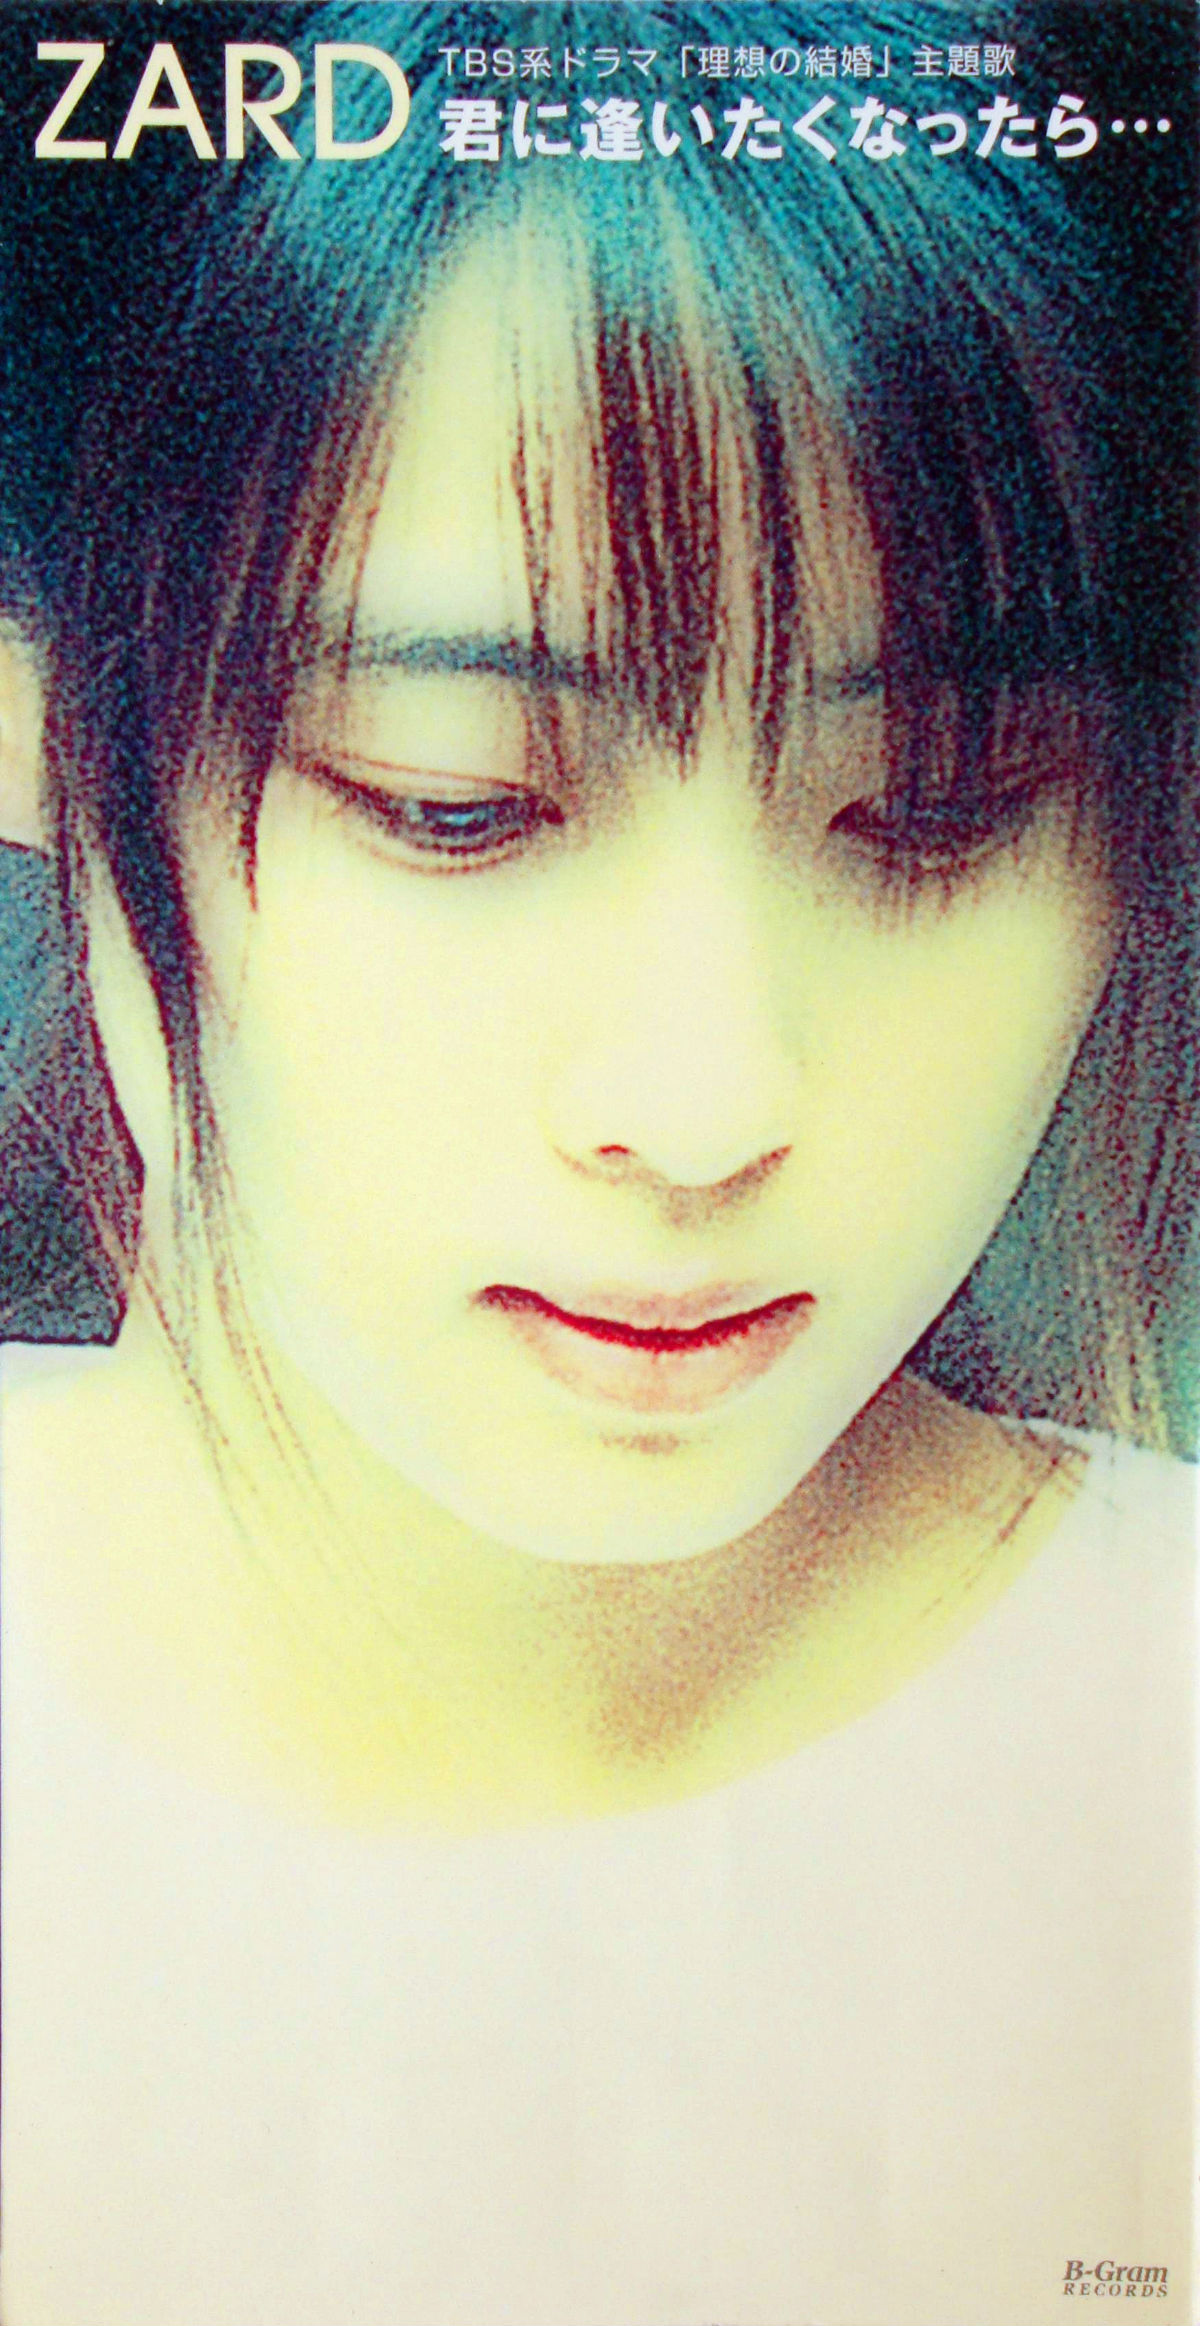
\includegraphics[width=0.3\textwidth]{S20.jpg}}

\ruby{君}{きみ}に\ruby{逢}{あ}いたくなったら…

いつだってすぐに\ruby{飛}{と}んで\ruby{行}{ゆ}ける

\ruby{壊}{こわ}れやすいものだからこそ

\ruby{大切}{たいせつ}にしたいと\ruby{思}{おも}う
\\

それでもあんな\ruby{出逢}{であ}いは\ruby{二度}{にど}とないよね

\ruby{悪}{わる}ぶったって

\ruby{人}{ひと}の\ruby{良}{よ}さそうな\ruby{瞳}{ひとみ}はかくせない

\ruby{遠}{とお}い\ruby{将来}{しょうらい}がこんなに

\ruby{早}{はや}く\ruby{来}{く}るとは \ruby{思}{おも}わなかった

\ruby{本当}{ほんとう}に\ruby{私}{わたし}でいいのかゆっくり\ruby{考}{かんが}えて…
\\

\ruby{君}{きみ}に\ruby{逢}{あ}いたくなったら…

いたずらな\ruby{笑顔}{えがお}を\ruby{想}{おも}い\ruby{出}{だ}す

「\ruby{大丈夫}{だいじょうぶ}だよ」という\ruby{君}{きみ}の\ruby{言葉}{ことば}が

\ruby{一番}{いちばん}\ruby{大丈夫}{だいじょうぶ}じゃない
\\

きっと\ruby{運命}{うんめい}が\ruby{二人}{ふたり}の

\ruby{味方}{みかた}をしてくれるでしょう

\ruby{我}{わ}がままじゃない きらいだからじゃないわかって
\\

\ruby{君}{きみ}に\ruby{逢}{あ}いたくなったら…

その\ruby{日}{ひ}までガンバル\ruby{自分}{じぶん}でいたい

これが\ruby{最初}{さいしょ}で\ruby{最後}{さいご}の\ruby{恋}{こい}に

なればいいなと\ruby{思}{おも}う
\\

\ruby{青}{あお}く\ruby{暮}{く}れかけた\ruby{街}{まち}\ruby{並}{な}み

また\ruby{思}{おも}い\ruby{切}{き}り\ruby{騒}{さわ}ごうね

}